\chapter{Thiết kế và Triển khai\label{chapter:design}}

\section{Đặc tả dùng chung: chuẩn công bằng}
\label{sec:fairness}
Trước khi viết bất kỳ mã nào, một đặc tả đã được đóng băng, và không phần nào trong đó gọi tên một ngôn ngữ.
Đặc tả cố định API công khai, máy trạng thái UE, cấu trúc dữ liệu và thuật toán đứng sau chúng
(bản đồ băm phân mảnh theo mã định danh UE, ví dụ), mức chi tiết của khóa và
phân mảnh, và mô hình đồng thời. Cả hai triển khai tuân theo đặc tả. Điều đó giữ cho
so sánh là so sánh hai ngôn ngữ, chứ không phải hai thiết kế hay hai mức kỹ năng. Đặc tả
là một sản phẩm độc lập, và là biện pháp kiểm soát chính chống
thiên lệch triển khai.

\section{Mô hình khái niệm và thiết kế đồng thời}\label{sec:concurrency}
Hai triển khai được xây dựng theo đặc tả dùng chung, và chúng làm cùng một việc: một
bản C++ hiện đại (C++23, STL, RAII, luồng chuẩn) và một bản Rust (bộ công cụ ổn định,
mô hình bộ nhớ dựa trên ownership, đồng thời an toàn). Cả hai dùng một mô hình đồng thời, mô tả là
\emph{không chia sẻ, một luồng cho mỗi shard}, cách mà RAN L3 thực tế chia trạng thái UE. Mô hình async và
mô hình dựa trên luồng không bao giờ được trộn, và đó là có chủ ý.

Không gian mã định danh UE được chia thành $N_{\text{shards}}$ shard, và mỗi shard thuộc về
đúng một luồng worker. Tám là mặc định. Chiến dịch đo ghim bảy thay vì, để
mỗi worker và mỗi producer sở hữu một trong các lõi được ghim, như
Mục~\ref{sec:testbed} ghi lại. Chỉ worker sở hữu đọc hoặc thay đổi ngữ cảnh của shard mình.
Worker do đó không chia sẻ trạng thái có thể thay đổi, và dữ liệu ngữ cảnh không cần khóa. Caller (các
luồng bộ tạo tải) không chạm trực tiếp vào trạng thái ngữ cảnh. Chúng gửi thông điệp yêu cầu vào
hàng đợi MPSC có giới hạn của một shard, rồi chờ trên tay cầm hoàn tất dùng một lần
mà worker ghi kết quả vào. Hàng đợi là \emph{có giới hạn và
chặn}. Khi hàng đợi của một shard đầy, gửi yêu cầu bị chặn cho đến khi có chỗ trống. Đó là điều
tạo ra độ trễ xếp hàng thực tế khi quá tải, và cũng là điều làm độ trễ đuôi
quan sát được, vì chính sách bỏ yêu cầu thay vì chặn sẽ che giấu
quá tải. Yêu cầu tới cùng một shard chạy nghiêm ngặt theo thứ tự vào trước ra trước.

Cấu trúc này cho so sánh đồng thời an toàn có thứ để đo. Cơ chế
được thử nghiệm là hàng đợi, bàn giao hoàn tất, và chuyển ownership của mỗi yêu cầu, chứ không phải
xung đột khóa. Một phần trạng thái có thể thay đổi được chia sẻ được phép: một bộ đếm nguyên tử ghi
số thứ tự hoạt động theo ngữ cảnh. Nó chỉ là ghi sổ, và không nhánh luồng điều khiển
phụ thuộc giá trị của nó. Độ trễ được đo trên toàn đường đi, từ thời điểm gửi dự kiến đến hoàn tất,
nên nó bao gồm độ trễ xếp hàng khi có tải và bao phủ cùng một vòng qua luồng trên cả hai
bên. Mục~\ref{sec:budget} sau đây tách số liệu thành phần ngôn ngữ thực thi và
phần hệ điều hành đảm nhiệm. Hình~\ref{fig:arch} cho thấy luồng dữ liệu, và
Hình~\ref{fig:reqlifecycle} truy vết một thao tác qua đó theo trình tự.

\begin{figure}[ht]
\centering
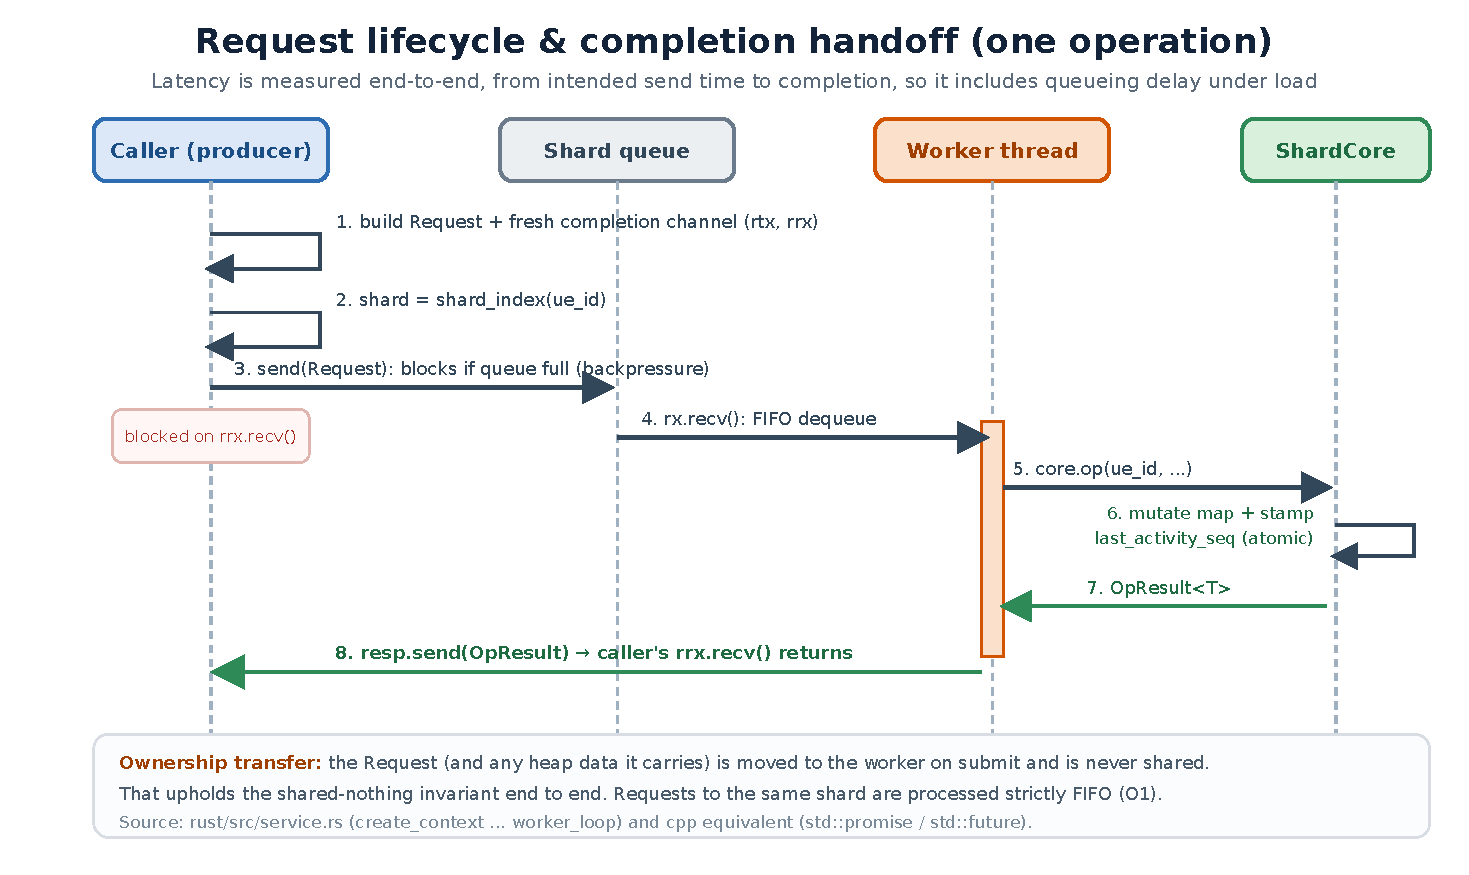
\includegraphics[width=0.78\linewidth]{diagrams/pdf/04_request_lifecycle_sequence.pdf}
\caption[Đường đi end-to-end của một thao tác]{Đường đi end-to-end của một thao tác và bàn giao hoàn tất. Caller xây dựng
một yêu cầu với tay cầm hoàn tất dùng một lần, định tuyến theo \texttt{shard\_index(ue\_id)} tới
hàng đợi có giới hạn của shard sở hữu (chặn nếu đầy), và chờ. Worker duy nhất của shard
dequeue theo thứ tự FIFO, thực thi thao tác trên store chỉ mình sở hữu, và ghi
kết quả trở lại tay cầm hoàn tất. Ownership của yêu cầu được chuyển cho worker khi
gửi và không bao giờ chia sẻ. Độ trễ được đo trên toàn đường đi.\label{fig:reqlifecycle}}
\end{figure}

\begin{figure}[ht]
\centering
\begin{tikzpicture}[
    font=\small,
    prod/.style={draw, rounded corners, minimum width=2.0cm, minimum height=0.66cm, fill=blue!8},
    queue/.style={draw, minimum width=2.5cm, minimum height=0.66cm, fill=gray!12},
    worker/.style={draw, rounded corners, minimum width=2.1cm, minimum height=0.66cm, fill=red!8},
    store/.style={draw, cylinder, shape border rotate=90, aspect=0.25, minimum width=1.5cm, minimum height=0.85cm, fill=green!8},
    lane/.style={draw, dotted, rounded corners, inner sep=7pt},
    >={Stealth[length=2.4mm]}
  ]
  % producers, grouped in one box to avoid a tangle of crossing arrows
  \node[prod] (p1) at (0,1.3)  {Producer 1};
  \node[prod] (p2) at (0,0.0)  {Producer 2};
  \node[prod] (p3) at (0,-1.3) {Producer $m$};
  \begin{scope}[on background layer]
    \node[draw, dashed, rounded corners, fill=blue!3, fit=(p1)(p2)(p3), inner sep=6pt] (pg) {};
  \end{scope}
  \node[font=\scriptsize] at (0,-2.15) {bộ tạo tải};

  % two representative shard lanes; spacing leaves room for the inline edge labels
  \node[queue] (q1) at (5.2,1.3)   {hàng đợi MPSC};
  \node[worker](w1) at (8.9,1.3)   {Worker 1};
  \node[store] (s1) at (12.0,1.3)  {Shard 1};
  \node[queue] (qn) at (5.2,-1.3)  {hàng đợi MPSC};
  \node[worker](wn) at (8.9,-1.3)  {Worker $N$};
  \node[store] (sn) at (12.0,-1.3) {Shard $N$};
  \begin{scope}[on background layer]
    \node[lane, fit=(q1)(s1)] (lane1) {};
    \node[lane, fit=(qn)(sn)] (lanen) {};
  \end{scope}
  \node[font=\scriptsize] at (8.35,2.35) {luồng sở hữu shard: không trạng thái chia sẻ, không khóa};

  % submit: producer group -> each shard queue, routed by hash
  \node[font=\scriptsize, align=center, fill=white, inner sep=2pt] at (2.85,0) {định tuyến theo\\ hash(\texttt{ue\_id})};
  \draw[->] (pg.east) -- (q1.west) node[midway, above, sloped, font=\scriptsize]{gửi};
  \draw[->] (pg.east) -- (qn.west) node[midway, below, sloped, font=\scriptsize]{gửi};

  % within-lane flow
  \draw[->]  (q1) -- node[above, font=\scriptsize]{FIFO} (w1);
  \draw[->]  (qn) -- node[above, font=\scriptsize]{FIFO} (wn);
  \draw[<->] (w1) -- node[above, font=\scriptsize]{sở hữu} (s1);
  \draw[<->] (wn) -- node[above, font=\scriptsize]{sở hữu} (sn);

  % one-shot completion: clean orthogonal return path below everything
  \draw[->, dashed, rounded corners=4pt]
      (wn.south) -- ++(0,-0.75) -- (1.4,-2.9) -- ($(pg.south east)+(-0.4,0)$);
  \node[font=\scriptsize] at (5.9,-3.05) {hoàn tất một lần (kết quả $\rightarrow$ producer đang chờ)};
\end{tikzpicture}
\caption[Kiến trúc không chia sẻ, một luồng cho mỗi shard]{Kiến trúc không chia sẻ, một luồng cho mỗi shard. Producer gửi thông điệp yêu cầu tới
hàng đợi MPSC có giới hạn, chặn của một shard (chọn bằng hash ghim của \texttt{ue\_id}) và chờ
trên tay cầm hoàn tất dùng một lần. Mỗi shard chỉ được đọc và ghi bởi đúng một luồng worker,
nên không có khóa trên trạng thái ngữ cảnh. Chặn khi hàng đợi đầy là điều làm quá tải
quan sát được như độ trễ đuôi.\label{fig:arch}}
\end{figure}

\section{Lựa chọn kiến trúc và ngăn xếp công nghệ}
Bên C++ dùng CMake với Ninja, thư viện chuẩn, và \texttt{std::thread}. Bên
Rust dùng Cargo và bộ công cụ ổn định. Cả hai liên kết cùng một bộ cấp phát bộ nhớ, điều đó giữ
so sánh về hai ngôn ngữ chứ không phải hai bộ cấp phát: C++ liên kết
\texttt{jemalloc} của hệ thống, và Rust cài một bộ cấp phát toàn cục \texttt{jemalloc} (từ
\texttt{tikv-jemallocator}). Mỗi bên cũng giữ một bản build với bộ cấp phát hệ thống làm đối chứng.
Độ trễ đi qua cùng thuật toán histogram HDR (HDR)~\cite{tene_hdrhistogram} trên cả hai bên, cấu hình giống nhau (phạm vi
$[1\,\text{ns}, 3.6\,\text{s}]$, ba chữ số có nghĩa). Rust dùng crate
\texttt{hdrhistogram} chuẩn. C++ dùng bản port header-only của cùng thuật toán gom nhóm,
được kiểm tra với phân phối đã biết. Tối ưu build được khớp gần nhất mà hai
bộ công cụ cho phép, nên profile release của Rust được ghim ở \texttt{opt-level~=~2} so với
build C++ \texttt{-O2}.

\section{Chi tiết triển khai}\label{sec:impldetails}
\label{sec:impl}
Cả hai triển khai tuân theo đặc tả đóng băng từng trường, và cả hai đủ nhỏ
để đọc từ đầu đến cuối. Lõi C++ là $\CppRawLines$ dòng trên tám header và hai
translation unit. Lõi Rust là $\RustRawLines$ dòng trên tám module. Bỏ dòng trống
và comment còn $\CppNloc$ và $\RustNloc$. Cả hai số mô tả build mà
chiến dịch thực sự đo. Một flag build bật hai thăm dò gán như Mục~\ref{sec:idioms}, và các khối điều kiện chọn chúng được bỏ khỏi số liệu,
vì đếm chúng sẽ mô tả không phải build được so sánh cũng không phải thăm dò.

Bản Rust do đó lớn hơn, $\RawRise\%$ theo dòng thô và
$\NlocRise\%$ theo dòng mã. Điều đó nên nằm trong văn bản chứ không phải chú thích cuối trang, vì hai lý do.
Số dòng là một trong các proxy chất lượng phần mềm mà nghiên cứu này đặt ra để thu thập. Và
khác biệt không phải dư thừa ngẫu nhiên: nó là kết quả ròng của nhiều điểm bắt buộc kéo theo chiều
ngược nhau, mà Mục~\ref{sec:idioms} phân tích từng file. Phần còn lại của mục này
đi từ mô hình dữ liệu ra cơ chế đồng thời, và báo cáo chi phí mỗi
phân kỳ buộc theo ngôn ngữ khi nó xuất hiện.

\subsection{Ngữ cảnh UE và máy trạng thái}\label{sec:uecontext}
Mỗi ngữ cảnh UE lưu mã định danh, trạng thái vòng đời (enumeration bốn giá trị
\texttt{Idle}, \texttt{Connected}, \texttt{Reconfiguring}, \texttt{Released}), cell phục vụ,
mã giao dịch RRC, một ngữ cảnh bảo mật giả 32 byte, danh sách động tối đa tám data
radio bearer, và hai bộ đếm (số thông điệp xử lý và số thứ tự hoạt động). Danh sách data
radio bearer cố ý là container có thể mở rộng (\texttt{std::vector} / \texttt{Vec})
chứ không phải mảng cố định, để nghiên cứu bộ cấp phát (RQ3) quan sát cấp phát
thực tế theo ngữ cảnh. Đọc trả về bản sao bất biến (\texttt{UeContextView}) sao chép ra từ
worker, không phải tham chiếu vào trạng thái shard đang sống. Điều đó giữ cam kết không chia sẻ
và giữ hai triển khai giống nghĩa hoàn toàn.
Hình~\ref{fig:datamodel} cho thấy bản ghi và đường đọc đầy đủ.

Khai báo trường giống hệt không tạo ra object giống hệt. Đo trên
máy đánh giá, \texttt{UeContext} chiếm $\CppUeCtxBytes$~byte trong C++ và chỉ
$\RustUeCtxBytes$~byte trong Rust.
Chính sách bố cục giải thích toàn bộ. C++ đảm bảo member dữ liệu không tĩnh nằm
theo thứ tự khai báo, nên enumeration một byte \texttt{state} giữa
mã định danh tám byte và cell id bốn byte buộc $\CppUeCtxStatePad$~byte padding, và
khóa bảo mật 32 byte, kết thúc ở offset $\CppUeCtxKeyEnd$, buộc thêm $\CppUeCtxKeyPad$ trước vector bearer căn tám byte. Rust không có chú thích \texttt{\#[repr(C)]} ở đây, nên có thể sắp xếp lại
trường, và nó làm vậy. Nó gom các scalar nhỏ và cả hai lỗ hổng biến mất.

Đặc tả không cố xóa khác biệt đó, và lý do cần nói rõ.
Ghim bố cục Rust bằng \texttt{\#[repr(C)]} sẽ phạt Rust chỉ vì tuân thủ
quy tắc padding của C++. Sắp xếp lại khai báo C++ thủ công sẽ là tối ưu mà
đặc tả không yêu cầu bên nào. Khoảng cách do đó được ghi là hiệu ứng cấp ngôn ngữ và
sau đó được giới hạn. Với $\SweepUes$ UE hoạt động mà sweep dùng, khoảng $\UeCtxGapBytes$ byte
tương đương khoảng $\UeCtxGapTotalKB$~kB. RSS được đo bằng megabyte, nên điều này
không ảnh hưởng so sánh RQ3.

\begin{figure}[ht]
\centering
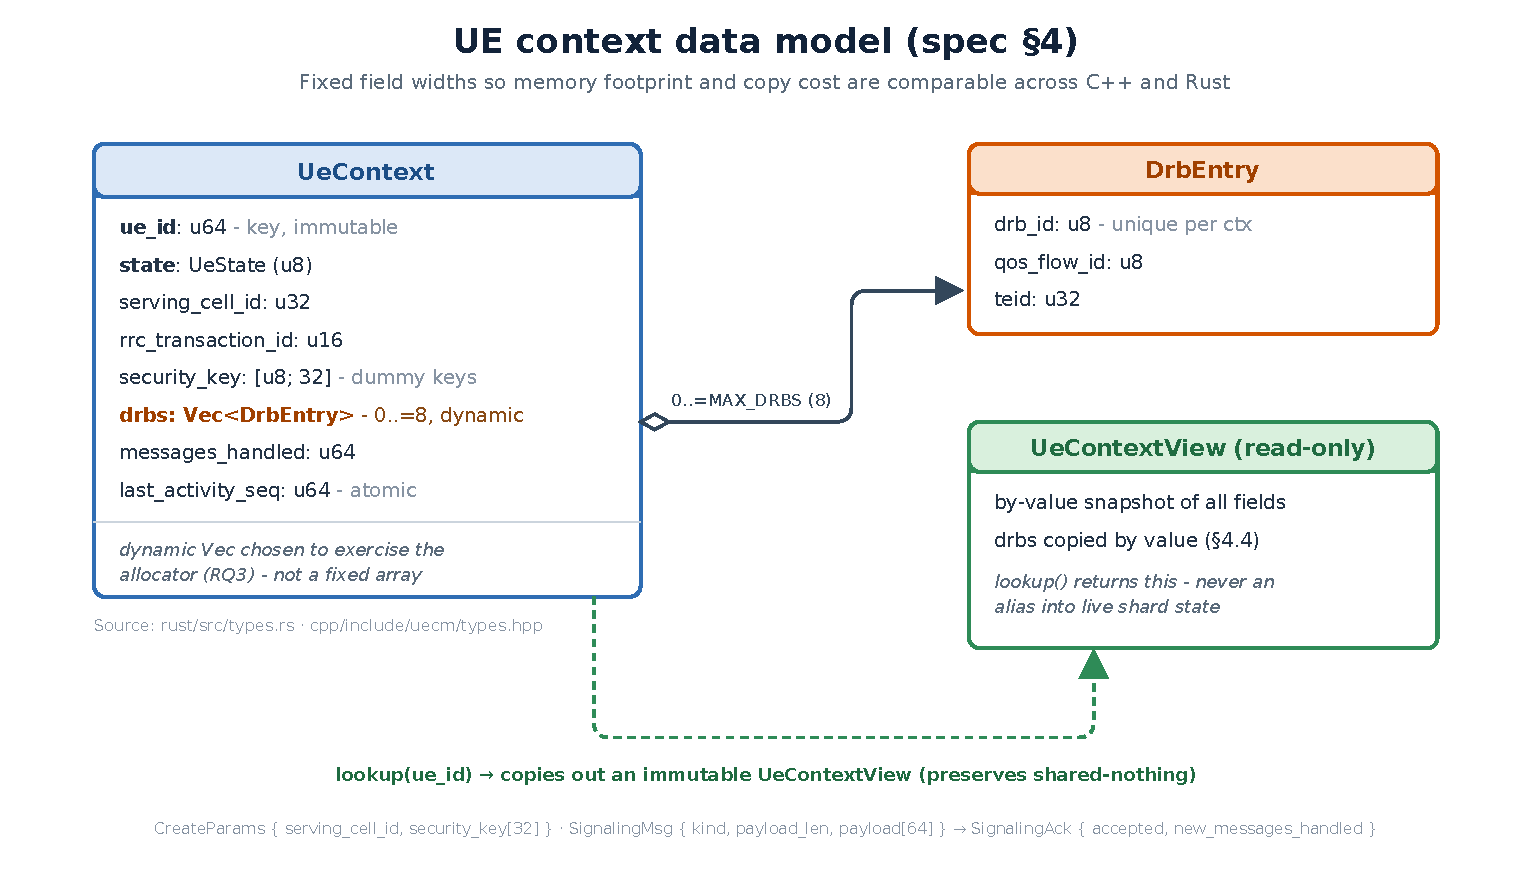
\includegraphics[width=0.72\linewidth]{diagrams/pdf/05_data_model.pdf}
\caption[Mô hình dữ liệu ngữ cảnh UE dùng chung]{Mô hình dữ liệu ngữ cảnh UE dùng chung cho cả hai triển khai. Chiều rộng trường được cố định để
dấu chân bộ nhớ và chi phí sao chép có thể so sánh giữa ngôn ngữ. Danh sách data-radio-bearer là
\texttt{Vec}/\texttt{std::vector} động có chủ ý, để kích hoạt bộ cấp phát cho RQ3.
\texttt{lookup} trả về \texttt{UeContextView} bất biến sao chép theo giá trị chứ không phải
alias vào trạng thái shard đang sống, giữ cam kết không chia sẻ.\label{fig:datamodel}}
\end{figure}

Bản ghi được điều khiển bởi vòng đời của Hình~\ref{fig:fsm}. Mỗi thao tác là một
chuyển trạng thái có bảo vệ, và Bảng~\ref{tab:transitions} cho bảng triển khai đầy đủ.
Hai tính chất giữ ở mọi nơi, và chúng là điều làm hai triển khai có thể so sánh từng
thao tác. Thứ nhất, mỗi thao tác kiểm tra trước khi thay đổi bất cứ gì. Chuỗi bảo vệ xác thực
mã định danh, tìm ngữ cảnh, kiểm tra trạng thái, và trả \texttt{OpError} khớp
trước khi chạm trường nào. Thao tác bị từ chối do đó để ngữ cảnh
bit-identical với trước đó. Thứ hai, không thao tác nào có thể thành công một phần, vì mỗi thao tác chỉ
thực hiện tối đa một đột biến sau bảo vệ cuối.

Hai hành vi cần nói rõ, vì bảng che chúng. Trạng thái
\texttt{Released} thực sự không được lưu. \texttt{release\_context} xóa entry
khỏi map shard hoàn toàn, nên \texttt{Released} chỉ là nhãn đi qua trong
đặc tả chứ không phải giá trị triển khai có thể bị bắt khi nghỉ. Lần
release thứ hai do đó trả \texttt{NotFound} chứ không phải \texttt{InvalidState}.
Trường hợp khác là \texttt{abort\_reconfigure}. Nó khôi phục \emph{trạng thái} về
\texttt{Connected}, nhưng không khôi phục serving cell mà \texttt{begin\_reconfigure}
đã ghi đè bằng mục tiêu handover. Đó là đơn giản hóa có chủ ý, vì mô hình không
lưu cell trước handover để rollback. Vẫn là cam kết ngữ nghĩa chứ không phải sơ suất,
và cả hai triển khai làm giống nhau, điều bộ parity của
Mục~\ref{sec:parity} kiểm tra.

\begin{table}[H]
\centering
\small
\caption[Bảng chuyển trạng thái triển khai]{Bảng chuyển trạng thái triển khai, giống hệt ở cả hai ngôn ngữ. Mọi thao tác
còn trả \texttt{InvalidArgument} cho \texttt{ue\_id} bằng không, và thao tác bị từ chối
để ngữ cảnh không thay đổi. \texttt{Released} không bao giờ được lưu: release xóa
entry.\label{tab:transitions}}
\begin{tabular}{@{}l l l R{0.31\linewidth}@{}}
\hline\hline
Thao tác & Trạng thái yêu cầu & Trạng thái kết quả & Lỗi \\
\hline
\texttt{create\_context}       & ngữ cảnh không có   & \texttt{Idle}          & \texttt{AlreadyExists}, \texttt{CapacityExceeded} \\
\texttt{setup\_connection}     & \texttt{Idle}          & \texttt{Connected}     & \texttt{NotFound}, \texttt{InvalidState} \\
\texttt{handle\_signalling}     & \texttt{Connected}     & \texttt{Connected}     & \texttt{NotFound}, \texttt{InvalidState} \\
\texttt{add\_drb}              & \texttt{Connected}     & \texttt{Connected}     & \texttt{NotFound}, \texttt{InvalidState}, \texttt{CapacityExceeded}, \texttt{AlreadyExists} \\
\texttt{begin\_reconfigure}    & \texttt{Connected}     & \texttt{Reconfiguring} & \texttt{NotFound}, \texttt{InvalidState} \\
\texttt{complete\_reconfigure} & \texttt{Reconfiguring} & \texttt{Connected}     & \texttt{NotFound}, \texttt{InvalidState} \\
\texttt{abort\_reconfigure}    & \texttt{Reconfiguring} & \texttt{Connected}     & \texttt{NotFound}, \texttt{InvalidState} \\
\texttt{release\_context}      & mọi trạng thái sống   & entry bị xóa           & \texttt{NotFound} \\
\texttt{lookup}                & mọi trạng thái sống   & không thay đổi              & \texttt{NotFound} \\
\hline
\end{tabular}
\end{table}

\subsection{Phân mảnh, store và hàng đợi có giới hạn}
Cả hai bên ghim hashing, để hasher của thư viện chuẩn không trở thành lợi thế
ngôn ngữ ngẫu nhiên. Gán shard chạy \texttt{ue\_id} qua finalizer SplitMix64,
ba vòng xor-shift và nhân với hằng
\texttt{0xBF58476D1CE4E5B9} và \texttt{0x94D049BB133111EB}, rồi giảm modulo số
shard. Finalizer quan trọng vì workload vẽ mã định danh tuần tự, và modulo
thuần sẽ ánh xạ chúng lên shard theo mẫu lặp cố định. Xáo trộn mã định danh trước
làm tải đều mỗi shard ở cả hai ngôn ngữ theo cấu trúc, không phải may mắn.

Container mỗi shard là hash map chuẩn của mỗi ngôn ngữ (\texttt{std::unordered\_map} /
\texttt{std::collections::HashMap}), nhưng hasher mặc định bị bỏ qua. Chúng khác quá nhiều
để giữ nguyên. \texttt{std::hash<uint64\_t>} của C++ thường là hàm identity, trong khi
\texttt{SipHash-1-3} mặc định của Rust mạnh về mật mã và tương ứng chậm hơn.
Giữ cả hai sẽ đo lựa chọn thư viện chuẩn, không phải ngôn ngữ. Cả hai map do đó
được key qua hash FNV-1a 64 bit ghim trên tám byte little-endian của
mã định danh, và một test kiểm tra \texttt{BuildHasher} của Rust tạo digest bit-identical
với \texttt{fnv1a\_64} tham chiếu.

Cả hai map reserve capacity ban đầu $4\,096$ entry khi khởi động để đo ổn định
không bị nhiễu bởi rehash. Cấu hình còn lại cũng chia sẻ:
mặc định tám shard, giới hạn hàng đợi
$1\,024$ yêu cầu mỗi shard, tối đa tám bearer và payload signalling 64 byte mỗi
ngữ cảnh, và giới hạn $200\,000$ ngữ cảnh mỗi shard. Chỉ số shard được thay từ
mặc định, và chỉ bởi chiến dịch, ghim để khớp lõi được cấp.

Hàng đợi chặn có giới hạn là nơi hai thư viện chuẩn phân kỳ rõ nhất. Rust
cung cấp nguyên thủy đặc tả yêu cầu. \texttt{sync\_channel(capacity)} là
kênh MPSC có giới hạn mà \texttt{send} chặn khi hàng đợi đầy và \texttt{recv} chặn khi rỗng, đúng
backpressure cần thiết trong một lời gọi. Thư viện chuẩn C++, tới C++23, không có
hàng đợi chặn có giới hạn. Cùng ngữ nghĩa do đó được ghép thủ công từ
\texttt{mutex}, hai \texttt{condition\_variable} và \texttt{std::queue}, trong class $45$
dòng.

Điểm so sánh không phải C++ viết kém. Nó ngắn, dùng
dạng predicate của \texttt{wait} để xử lý wakeup giả đúng, và
thả khóa trước khi notify. Điểm là nó tồn tại. Mỗi dòng
là nơi lỗi đồng thời có thể lọt vào. Và lập luận đúng đắn cho nó phụ thuộc
tác giả, không phải compiler hay thư viện: hai condition variable không bị nhầm,
predicate khớp notification, không mất wakeup. Đây là
cùng bất đối xứng mà nghiên cứu tiêm lỗi Chương~\ref{chapter:eval} đo, xuất hiện ở đây
trong mã thường không có lỗi cố ý thay vì trong bug được đặt vào.

\subsection{Yêu cầu, phản hồi và vòng đời dịch vụ}\label{sec:tagged}
\label{sec:request}
Kiểu thông điệp qua hàng đợi là phân kỳ buộc thứ hai. Rust mô hình
yêu cầu là \texttt{enum} với một variant cho mỗi
thao tác. Mỗi variant mang đúng tham số của nó cộng tham số \texttt{Sender}
theo đúng kiểu kết quả của thao tác đó. C++ không có enumeration mang payload
theo idiom chuẩn dùng ở đây, nên yêu cầu là struct có tag. Nó giữ
discriminant \texttt{OpKind} cùng \emph{mọi} trường tham số mà bất kỳ thao tác nào có thể cần,
ghép với một \texttt{std::promise}. Kiểu giá trị của promise do đó phải là
\texttt{std::variant} trên cả bốn kiểu kết quả có thể.

Điều này có ba hệ quả đo được. Thứ nhất là kích thước. \texttt{Request} là $\CppRequestBytes$~byte
trong C++ so với $\RustRequestBytes$ trong Rust, vì struct C++ luôn mang tham số create, thông điệp signalling
$\SignalingMsgBytes$ byte, entry bearer, và tham số reconfiguration, dù
thao tác đang chạy có dùng hay không. Enum Rust được size theo variant lớn nhất
riêng. Với mặc định tám shard giữ tối đa $1\,024$ yêu cầu mỗi shard, occupancy đầy nghĩa là khoảng $\CppQueueResidentMB$~MB
lưu trữ yêu cầu trong hàng đợi so với $\RustQueueResidentMB$~MB. Hệ quả thứ hai là chi phí sao chép
trả trên mỗi gửi, vì trường không dùng được khởi tạo mặc định và move cùng
trường dùng.

Thứ ba quan trọng nhất cho luận điểm luận văn, và là khoảng trống an toàn kiểu.
Caller C++ phải khôi phục kết quả có kiểu từ variant bằng
\texttt{std::get<OpResult<T>>}, ném \texttt{std::bad\_variant\_access} nếu worker
ghi alternative caller không mong đợi. Exception đó không thể xảy ra trong
mã hiện tại, vì mỗi \texttt{OpKind} được xử lý bởi đúng một nhánh và nhánh đó
lưu alternative khớp. Nhưng invariant đứng sau nó được duy trì bằng đọc hai
file, không phải compiler. Rust thiết lập cùng invariant theo cấu trúc. Sender nhúng
trong mỗi variant đã có kiểu, nên không có union phản hồi, không cần unwrap, và không
dispatch runtime trên đường trả.

Khởi động dịch vụ cấp phát shard, spawn một luồng worker mỗi shard, và giao
worker sở hữu duy nhất store của mình. Đường yêu cầu sau đó là đường Mục~\ref{sec:concurrency} mô tả. Shutdown là nửa tinh tế hơn. Nó phải dừng
worker bị chặn trên hàng đợi rỗng mà không bỏ yêu cầu còn
đang chạy. Cả hai triển khai giải bằng sentinel \texttt{Stop} in-band.
Một yêu cầu \texttt{Stop} được đẩy vào hàng đợi mỗi shard, và vì hàng đợi nghiêm ngặt
FIFO, mọi yêu cầu đã xếp trước nó chạy hoàn tất trước khi worker
thấy sentinel và trả về. Không cần flag đóng riêng, timeout, hay API drain,
và không tay cầm hoàn tất bị bỏ chưa fulfill. Luồng worker sau đó được join, nên shutdown
chỉ trả về khi mọi shard thực sự dừng.

Cả hai ngôn ngữ gắn điều này với hủy object, và cơ chế là một trong vài chỗ
hai bên gần giống hệt: destructor C++ gọi \texttt{shutdown()}, và
triển khai \texttt{Drop} của Rust làm tương tự, nên dịch vụ ra khỏi phạm vi không thể để
luồng detached. Cả hai chống gọi đôi bằng flag \texttt{running},
làm shutdown idempotent.

Khoảng giữa hai lời gọi là điều kiện tiên quyết cho mọi thao tác, và được viết
một lần. Thao tác gửi trước \texttt{start()} hoặc sau \texttt{shutdown()} là lỗi caller
chứ không phải điều kiện runtime, nên được báo ngoài band và không mở rộng tập
\texttt{OpError} đóng của Mục~\ref{sec:parity}. C++ ném \texttt{std::logic\_error} và Rust
panic. Nói rõ không phải hình thức. Đặc tả cấm lời gọi từ
đầu, không triển khai nào kiểm tra, và trong khoảng trống đó hai ngôn ngữ không thất bại giống nhau.
Sự kiện được báo cùng kết quả an toàn Mục~\ref{sec:safetyresults}, vì
lỗi trong mã viết để đúng mang bằng chứng mà lỗi tiêm không thể.

Một mảnh kỷ luật ownership nữa giữ invariant không chia sẻ từ đầu đến cuối. Yêu cầu
được move vào hàng đợi chứ không sao chép, và mang tay cầm hoàn tất, nên
producer và worker không bao giờ cùng giữ tham chiếu dùng được tới cùng yêu cầu. C++ buộc
bằng làm \texttt{Request} chỉ move, tính chất tự động từ
\texttt{std::promise} chỉ move bên trong. Trong Rust nó theo move semantics thường, và
compiler từ chối mọi cố dùng yêu cầu sau khi gửi. Trạng thái có thể thay đổi chia sẻ duy nhất
trong cả hai triển khai là bộ đếm hoạt động nguyên tử. C++ giữ bằng tham chiếu, Rust là
\texttt{Arc<AtomicU64>} clone, và cả hai tăng bằng ordering relaxed vì không
nhánh theo giá trị.

\subsection{Điểm bắt buộc theo ngôn ngữ và chi phí hai lõi}
\label{sec:idioms}
Khi hai ngôn ngữ phải phân kỳ để đáp ứng cùng yêu cầu, phân kỳ được
ghi trong log điểm bắt buộc của đặc tả để được cân nhắc chứ không
lẫn vào kết quả. Bảng~\ref{tab:idioms} gom log đầy đủ, và
các mục trước đã định lượng hai mục có hệ quả đo được.

\begin{table}[H]
\centering
\small
\caption[Log điểm bắt buộc theo ngôn ngữ]{Log điểm bắt buộc: mọi điểm hai triển khai phân kỳ để
đáp ứng cùng yêu cầu đặc tả, với hệ quả đo được nếu có.\label{tab:idioms}}
\begin{tabular}{@{}R{0.20\linewidth} R{0.36\linewidth} R{0.36\linewidth}@{}}
\hline\hline
Vấn đề & C++ & Rust \\
\hline
Kiểu kết quả & \texttt{std::expected<T, OpError>} & \texttt{Result<T, OpError>} \\
Yêu cầu & struct có tag: discriminant cộng mọi trường tham số ($\CppRequestBytes$\,B) & \texttt{enum}, một variant mỗi thao tác, chỉ mang tham số riêng ($\RustRequestBytes$\,B) \\
Phản hồi & \texttt{std::variant} của bốn kiểu kết quả, caller unwrap bằng \texttt{std::get} & không cần: mỗi variant mang sender của kiểu kết quả riêng \\
Hàng đợi có giới hạn & \texttt{mutex} viết tay cộng hai \texttt{condition\_variable} ($\CppBoundedQueueLines$ dòng) & \texttt{sync\_channel(capacity)} \\
Hoàn tất & \texttt{std::promise} / \texttt{std::future} & \texttt{mpsc::channel()} mới mỗi yêu cầu \\
Map mỗi shard & \texttt{std::unordered\_map} với functor \texttt{FnvHash} & \texttt{HashMap} với \texttt{FnvBuildHasher} \\
Bộ đếm hoạt động & \texttt{std::atomic<uint64\_t>} giữ bằng tham chiếu & \texttt{Arc<AtomicU64>} clone vào mỗi worker \\
Tháo dỡ & destructor gọi \texttt{shutdown()} & \texttt{Drop} gọi \texttt{shutdown()} \\
Mức tối ưu & \texttt{-O2} & \texttt{opt-level = 2} \\
\hline
\end{tabular}
\end{table}

Log cũng giải thích khác biệt số dòng ở đầu mục này, và
nói nhiều hơn số ròng, vì đóng góp không cùng chiều.
Bảng~\ref{tab:loc} chia khoảng $\LocGap$ dòng theo vấn đề. Rust
\emph{ngắn hơn} nhiều ở đúng một chỗ, hàng đợi có giới hạn, nơi không cần mã
so với $\CppBoundedQueueLines$ dòng C++. Nó dài hơn gần như mọi nơi khác, và
ba mục chiếm phần lớn phần dư.

Lớn nhất là module dịch vụ, vì lý do trên. Vì phản hồi C++ là một
\texttt{variant}, mọi thao tác công khai mười đi qua một helper \texttt{submit}
chia sẻ, và mỗi wrapper có kiểu co còn hai hoặc ba dòng. Sender có kiểu theo variant của Rust
không cho phép helper tương tự không dùng generic, nên mỗi thao tác lặp cùng chuỗi:
tạo kênh hoàn tất, dựng variant, gửi, nhận. Mục tiếp cho thấy trade-off rõ nhất, và là hashing. C++ đáp ứng
yêu cầu hasher của \texttt{std::unordered\_map} bằng functor năm dòng bọc
\texttt{fnv1a\_64}. Rust phải cung cấp toàn bộ apparatus trait, mỗi dòng
boilerplate, và đổi lại là hasher dispatch tĩnh, kiểm tra kiểu thay vì
callable theo hình thường. Mục thứ ba là cây module và danh sách re-export công khai,
việc C++ có miễn từ cấu trúc header.

Không phần nào là lỗi của bên nào, và không xuất hiện trong số liệu hiệu năng.
Đó là loại chi phí kỹ thuật mà log điểm bắt buộc tồn tại để phơi bày. Rust tiêu dòng nguồn
cho machinery trait và lặp tại call site, và đổi lại là cam kết
compiler có thể kiểm tra. Sau đó nó thu hồi phần lớn chi tiêu ở chỗ thư viện chuẩn
cung cấp nguyên thủy mà C++ không có.

Đếm dòng chỉ trả lời nửa câu hỏi reviewer của codebase sẽ hỏi,
vì nó co một dòng boilerplate và một dòng nhánh là cùng loại.
Bảng~\ref{tab:complexity} do đó thêm độ phức tạp cyclomatic, đo bằng
\texttt{lizard}~\cite{lizard} trên cả hai lõi. Một công cụ áp dụng cho cả hai ngôn ngữ làm
số liệu có thể so sánh, vì nó dùng cùng định nghĩa điểm quyết định mỗi bên.
Công cụ riêng mỗi ngôn ngữ sẽ đếm hơi khác. Hai đo lường sau đó
đi ngược chiều. Rust dài $\NlocRise\%$ hơn C++ theo dòng mã, nhưng
tổng cyclomatic complexity thấp $\CcnTotalDrop\%$, $\RustCcnTotal$ so với
$\CppCcnTotal$, trải trên hơi nhiều hàm ($\RustFuncs$ so với $\CppFuncs$). Cả hai
lõi đều không đòi hỏi theo ngưỡng thường, và cả hai có median complexity
mỗi hàm bằng một, nên số hàm ở đỉnh mang tổng hợp.

Đỉnh là nơi khác biệt nằm, và truy ngược phân kỳ đã mô tả,
không phải thứ rải mỏng. Hàm phức tạp nhất trong lõi C++ là
$\CppCcnMaxFn$ ở $\CppCcnMax$, hơn gấp đôi đối tác Rust $\RustCcnMax$. Nó
switch trên discriminant \texttt{OpKind} rồi lưu alternative khớp vào
\texttt{variant} phản hồi. Thiết kế struct có tag Mục~\ref{sec:tagged} do đó
gom toàn bộ dispatch và lập luận đúng đắn đi kèm vào một hàm nhiều nhánh.
Sender có kiểu theo variant của Rust loại bỏ dispatch đường trả hoàn toàn, nên
worker Rust không có gì tương đương unwrap. Trade-off sắc hơn số dòng
gợi ý. Dòng thêm Rust đổi lại bằng nhánh ở chỗ
nhánh khó review nhất. Và invariant \texttt{std::bad\_variant\_access} mà
Mục~\ref{sec:tagged} mô tả là duy trì bằng đọc hai file nằm trong
đúng hàm mà đo lường này đánh dấu.

\begin{table}[H]
\centering
\small
\caption[Proxy kích thước và cyclomatic complexity cho hai lõi]{Proxy kích thước và cyclomatic complexity cho hai lõi, đo bằng
\texttt{lizard}~\cite{lizard} áp dụng giống nhau cho cả hai ngôn ngữ. Driver benchmark, test,
runner conformance, seam FFI, và khối điều kiện thăm dò của
Mục~\ref{sec:idioms} bị loại. Chỉ mã so sánh mà hợp đồng parity ràng buộc được
đếm. Complexity là một cộng số điểm quyết định trong hàm. Số dòng là
NLOC theo \texttt{lizard}, cũng loại dòng chỉ có brace và preprocessor. Đó là
cùng đo lường trích ở đầu
Mục~\ref{sec:impldetails}.\label{tab:complexity}}
\begin{tabular}{@{}l r r@{}}
\hline\hline
Đo lường & C++ & Rust \\
\hline
Files & 10 & 8 \\
Functions & 37 & 42 \\
Lines of code (blank and comment lines excluded) & 517 & 621 \\
Total branching complexity & 95 & 83 \\
Mean complexity per function & 2.6 & 2.0 \\
Median complexity per function & 1 & 1 \\
Most complex function & 13 (\texttt{worker\_loop}) & 6 (\texttt{add\_drb})
\\
\hline
\end{tabular}
\end{table}

\begin{table}[H]
\centering
\small
\caption[Nguồn gốc khác biệt số dòng giữa hai lõi]{Nguồn gốc khoảng $\LocGap$ dòng giữa hai lõi, theo vấn đề (dòng thô,
bao comment. Số C++ gộp header và translation unit. Khối điều kiện thăm dò loại như
Mục~\ref{sec:impldetails}). Rust chỉ ngắn hơn
ở chỗ thư viện chuẩn cung cấp nguyên thủy C++ thiếu.\label{tab:loc}}
\begin{tabular}{@{}R{0.38\linewidth} r r r@{}}
\hline\hline
Vấn đề & C++ & Rust & $\Delta$ \\
\hline
Service (queues, workers, API) & $234$ & $291$ & $+57$ \\
Hashing (functor vs.\ trait pair) & $37$ & $70$ & $+33$ \\
Module tree and re-exports & $0$ & $26$ & $+26$ \\
Message types & $48$ & $67$ & $+19$ \\
Data model & $73$ & $85$ & $+12$ \\
Configuration & $18$ & $29$ & $+11$ \\
Shard core (state machine) & $182$ & $188$ & $+6$ \\
Error model & $32$ & $26$ & $-6$ \\
Bounded queue & $51$ & $0$ & $-51$
\\
\hline
Tổng                             & $\CppRawLines$ & $\RustRawLines$ & $+\LocGap$ \\
\hline
\end{tabular}
\end{table}

Một tính chất của lõi Rust không phải chi phí, và nó kết mục này vì là thứ
các chi phí trên mua được. Thư viện Rust chứa \emph{không} mã \texttt{unsafe}, và
được kiểm tra cơ học trên crate. Safe Rust do đó đảm bảo không data race cho lõi này ở
thời điểm biên dịch, qua trait \texttt{Send} và \texttt{Sync}. Store shard được một
worker sở hữu và không chia sẻ, kiểu yêu cầu được move qua ranh giới luồng, và
phần trạng thái thực sự chia sẻ là bộ đếm hoạt động nguyên tử. Không phần nào cần
sanitiser runtime để thiết lập, và không phần nào cần coverage test để giữ. Triển khai C++
không làm quản lý bộ nhớ thủ công ngoài container STL và không khóa tường minh
ngoài class hàng đợi, và được kiểm tra không data race dưới ThreadSanitizer.

Hai câu không phải cùng loại bằng chứng, và khác biệt đó là
luận điểm an toàn trung tâm của luận văn ở dạng nhỏ. Tính chất Rust là định lý về chương trình,
compiler giải quyết trên mọi build thường và bao mọi thực thi. Tính chất C++
là quan sát về các thực thi binary có instrument tình cờ chạy,
và phải được thiết lập lại sau mọi thay đổi, trên build hầu hết dự án không
chạy mặc định. Định lượng hai loại cam kết cách xa nhau là
mục đích nghiên cứu tiêm lỗi Chương~\ref{chapter:eval}.

\section{API công khai và ngữ nghĩa thao tác}
Cả hai triển khai expose cùng API nhỏ, theo vòng đời, theo đặc tả dùng chung,
nên bề mặt caller thấy giống hệt ngoài quy ước tên của mỗi ngôn ngữ.
Dịch vụ được tạo với số shard cố định và giới hạn hàng đợi mỗi shard.
Caller sau đó gọi thao tác ngữ cảnh, mỗi thao tác theo \texttt{ue\_id} mục tiêu: create,
setup, handle-signalling, add-bearer, reconfigure begin/complete/abort, release, và tra
trạng thái. Mỗi thao tác là \emph{total} và \emph{typed}. Nó trả giá trị thành công hoặc
\texttt{OpError} có kiểu từ enumeration đóng năm giá trị (\texttt{NotFound},
\texttt{AlreadyExists}, \texttt{InvalidState}, \texttt{CapacityExceeded} và
\texttt{InvalidArgument}). Thao tác bất hợp với trạng thái hiện tại của ngữ cảnh (Hình~\ref{fig:fsm}) trả lỗi khớp và để ngữ cảnh
không đổi. Nó không đột biến ngữ cảnh, và không báo thất bại ngoài band.

Lựa chọn quan trọng cho công bằng cũng như đúng đắn. Không triển khai nào dùng
exception hay mã lỗi làm kênh luồng điều khiển ẩn, nên chi phí và luồng điều khiển của
đường thất bại hiển nhiên và giống hệt hai bên. Điều đó cũng nghĩa là cùng vector conformance
(Mục~\ref{sec:parity}) có thể khẳng định đồng ý từng thao tác cả giá trị trả và
trạng thái kết quả.

\section{Kiểm tra tương đồng}
\label{sec:parity}
Toàn bộ so sánh dựa trên hai bản chức năng giống hệt, nên parity
được kiểm tra chứ không giả định. Bộ conformance trung lập ngôn ngữ viết vector test là
chuỗi thao tác với kết quả mong đợi và tóm tắt trạng thái sau. Runner
mỗi ngôn ngữ thực thi vector và xuất transcript một định dạng cố định, và
hai transcript được diff để đồng ý từng thao tác. Bộ có seed bao phủ toàn mô hình lỗi,
đường reconfiguration begin/complete/abort, data-radio-bearer đầy và tràn, và
tính quyết định gán shard. Cả hai triển khai hiện pass và đồng ý. Workload benchmark
thêm tín hiệu parity thứ hai, độc lập với thứ nhất. Với seed và quần UE hoạt động cho trước,
số đếm theo loại thao tác của workload mixed được kiểm tra giống hệt giữa
ngôn ngữ, xác nhận cả hai triển khai được điều khiển qua cùng đường mã.

Hai điều giới hạn điều đó thiết lập, và cả hai được trả lời chứ không nhượng bộ. Cross-diff hai triển khai không phân biệt ``cả hai đúng'' với ``cả hai sai
cùng cách'', và đó là chế độ thất bại mà đặc tả dùng chung và một tác giả làm
dễ nhất. Kết quả mong đợi trong vector viết tay cũng đến từ
đặc tả qua người viết triển khai. Triển khai thứ ba của
cùng đặc tả viết làm oracle độc lập. Nó viết bằng Python,
không chia sẻ mã với ngôn ngữ nào, và phải tái tạo mọi $\ConfHandOps$ kỳ vọng
suy ra tay trước khi được tạo kỳ vọng riêng. Sau đó nó tạo chuỗi thao tác ngẫu nhiên
dưới nhiều profile: vòng đời thực tế, chuỗi adversarial
nặng về chuyển trạng thái bất hợp, chuỗi ở giới hạn capacity, và chuỗi
stress gán shard. Mô hình tính mọi kết quả mong đợi. Chiến dịch
khoảng $\ConfGenOps$ thao tác tạo không có phân kỳ. Hai
triển khai đồng ý với nhau, và với cách đọc độc lập đặc tả, trên
chuỗi không ai chọn. Generator có seed và quyết định, nên mọi phân kỳ tương lai là
hồi quy tái lập vĩnh viễn chứ không phải giai thoại.

Ba kiểm tra nữa giới hạn bộ theo hướng khác. Ma trận chuyển trạng thái của đặc tả
được duyệt đầy đủ chứ không mẫu: mỗi thao tác áp lên ngữ cảnh ở
mọi trạng thái nó có thể chiếm. Mỗi trường hợp khẳng định lỗi chính xác, trạng thái kết quả khi thành công, và
không thay đổi trường khi thất bại, kể cả thứ tự ưu tiên lỗi đặc tả
để không thứ tự. Triển khai C++ sau đó chạy dưới AddressSanitizer, ThreadSanitizer
và UndefinedBehaviorSanitizer trên toàn bộ, và không báo gì. Điều đó quan trọng cho
công bằng. Safe Rust mang không data race và an toàn bộ nhớ theo cấu trúc, nên không
chạy sanitiser thì nhánh C++ tương đương sẽ dựa trên chưa thất bại thay vì
đã được kiểm tra. Miri, chạy trên bộ máy trạng thái Rust, cũng không báo
hành vi không định nghĩa. Thứ ba, phạm vi bộ được đo chứ không khẳng định, vì
kết quả âm từ sanitiser chỉ rộng bằng mã đã chạy. Coverage dòng của
thư viện C++ là $\CppLineCov\%$ và thư viện Rust $\RustLineCov\%$, và processor thao tác lõi
và facade dịch vụ của cả hai triển khai được bao phủ đầy đủ. Hai số không
so sánh nghiêm ngặt, vì \texttt{gcov} và \texttt{llvm-cov} không phân giải dòng thực thi giống nhau.
Trên vùng chi tiết hơn \texttt{llvm-cov} đếm, số Rust là $\RustRegionCov\%$.
Mỗi số giới hạn luận điểm về triển khai của nó.
